\documentclass[11pt,a4paper]{book}
% =====================================================================
% Preambuła książki naukowej wiernie wzorowana na „Mathematics for Machine
% Learning” (Deisenroth, Faisal, Ong):
%  - czcionka Times, czarno-biały skład, bez kolorowych ramek,
%  - definicje i twierdzenia: pogrubiony nagłówek w tekście, bez ramki,
%  - szare tło TYLKO dla przykładów,
%  - szeroki margines: podpisy rysunków, hasła (\haslo) i uwagi na marginesie,
%  - uwagi i intuicje jako kursywne „Uwaga.” zakończone znakiem ◊,
%  - nagłówek strony: numer + kursywny tytuł rozdziału / sekcji, bez linii.
% Wykresy powstają osobno w Pythonie (figures/) i wchodzą jako obrazy.
% =====================================================================
\usepackage[T1]{fontenc}
\usepackage[utf8]{inputenc}
\usepackage[polish]{babel}
\usepackage{mathptmx}              % Times + dopasowana matematyka
\usepackage{microtype}
\usepackage{amsmath,amssymb,amsthm,mathtools,bm}
\usepackage{booktabs,array}
\usepackage{graphicx}
\usepackage{xcolor}
\usepackage{enumitem}
\setlist[enumerate]{leftmargin=*,itemsep=2pt,topsep=3pt}
\setlist[itemize]{leftmargin=*,itemsep=2pt,topsep=3pt}

% ---------- układ strony: szeroki zewnętrzny margines ----------
\usepackage[a4paper,twoside,inner=2.4cm,textwidth=11.6cm,marginparsep=0.55cm,
  marginparwidth=4.9cm,top=2.7cm,bottom=2.9cm,headheight=14pt,headsep=0.9cm]{geometry}
\usepackage{sidenotes}             % \sidenote, \sidecaption, marginfigure, figure*
\definecolor{mmlgray}{gray}{0.94}  % jedyny „kolor” książki: szare tło przykładów

\usepackage{hyperref}
\hypersetup{colorlinks=true,linkcolor=black,citecolor=black,urlcolor=black,
  pdfauthor={},pdftitle={}}
\usepackage{cleveref}
\crefname{figure}{rys.}{rys.}\Crefname{figure}{Rysunek}{Rysunki}
\crefname{table}{tab.}{tab.}\Crefname{table}{Tabela}{Tabele}
\crefname{equation}{wzór}{wzory}\Crefname{equation}{Wzór}{Wzory}
\crefname{chapter}{rozdział}{rozdziały}\Crefname{chapter}{Rozdział}{Rozdziały}
\crefname{section}{sekcja}{sekcje}\Crefname{section}{Sekcja}{Sekcje}
\crefname{definicja}{def.}{def.}\Crefname{definicja}{Definicja}{Definicje}
\crefname{twierdzenie}{tw.}{tw.}\Crefname{twierdzenie}{Twierdzenie}{Twierdzenia}
\crefname{lemat}{lemat}{lematy}\Crefname{lemat}{Lemat}{Lematy}
\crefname{wniosek}{wniosek}{wnioski}\Crefname{wniosek}{Wniosek}{Wnioski}
\crefname{przyklad}{przykład}{przykłady}\Crefname{przyklad}{Przykład}{Przykłady}

\numberwithin{equation}{chapter}   % (2.94): numer rozdziału i wzoru

% ---------- nagłówki rozdziałów i sekcji (jak w MML: czarne, pogrubione) ----------
\usepackage[explicit]{titlesec}
\titleformat{\chapter}[hang]{\bfseries\fontsize{26}{30}\selectfont}{\thechapter}{0.9em}{#1}
\titleformat{name=\chapter,numberless}[hang]{\bfseries\fontsize{26}{30}\selectfont}{}{0pt}{#1}
\titlespacing*{\chapter}{0pt}{16pt}{34pt}
\titleformat{\section}{\large\bfseries}{\thesection}{0.8em}{#1}
\titleformat{\subsection}{\bfseries\itshape}{\thesubsection}{0.8em}{#1}
\titleformat{\paragraph}[runin]{\bfseries\itshape}{}{0pt}{#1.}
\titlespacing*{\section}{0pt}{2.8ex plus 1ex minus .2ex}{1.2ex plus .2ex}
\titlespacing*{\subsection}{0pt}{2.4ex plus 1ex minus .2ex}{1ex plus .2ex}

% ---------- nagłówki i stopki stron (numer + kursywny tytuł, bez linii) ----------
\usepackage{fancyhdr}
\pagestyle{fancy}
\fancyhf{}
\renewcommand{\headrulewidth}{0pt}
\renewcommand{\chaptermark}[1]{\markboth{#1}{}}
\renewcommand{\sectionmark}[1]{\markright{\thesection\ #1}}
\fancyhead[LE]{\thepage}
\fancyhead[RE]{\textit{\leftmark}}
\fancyhead[LO]{\textit{\rightmark}}
\fancyhead[RO]{\thepage}
\fancypagestyle{plain}{\fancyhf{}\fancyfoot[C]{\thepage}\renewcommand{\headrulewidth}{0pt}}

% ---------- spis treści: pogrubione rozdziały, bez kropek ----------
\usepackage{tocloft}
\renewcommand{\cfttoctitlefont}{\bfseries\fontsize{26}{30}\selectfont}
\renewcommand{\cftaftertoctitleskip}{24pt}
\renewcommand{\cftchapfont}{\bfseries}
\renewcommand{\cftchappagefont}{\bfseries}
\renewcommand{\cftdotsep}{\cftnodots}

% ---------- podpisy rysunków: mała czcionka, pogrubiona etykieta, w marginesie ----------
\captionsetup{font=footnotesize,labelfont=bf,justification=raggedright,
  singlelinecheck=off,skip=4pt}

% ---------- twierdzenia, definicje, przykłady ----------
\usepackage[most]{tcolorbox}
% nagłówek pogrubiony w tekście, bez ramki: „Definicja 2.10 (Nazwa).”
\newtheoremstyle{mmldef}{9pt}{9pt}{\normalfont}{0pt}{\bfseries}{.}{0.5em}
  {\thmname{#1}\ \thmnumber{#2}\thmnote{\ (#3)}}
\newtheoremstyle{mmlthm}{9pt}{9pt}{\itshape}{0pt}{\bfseries}{.}{0.5em}
  {\thmname{#1}\ \thmnumber{#2}\thmnote{\ (#3)}}
\theoremstyle{mmldef}
\newtheorem{definicja}{Definicja}[chapter]
\newtheorem{przyklad}{Przykład}[chapter]       % własna numeracja, jak w MML
\theoremstyle{mmlthm}
\newtheorem{twierdzenie}[definicja]{Twierdzenie}
\newtheorem{lemat}[definicja]{Lemat}
\newtheorem{wniosek}[definicja]{Wniosek}
\renewcommand{\qedsymbol}{$\blacksquare$}

% jedyna ramka: szare tło przykładów
\tcbset{mmlbox/.style={enhanced,breakable,sharp corners,frame hidden,boxrule=0pt,
  colback=mmlgray,left=8pt,right=8pt,top=5pt,bottom=5pt,
  before skip=11pt,after skip=11pt,before upper={\parindent0pt}}}
\tcolorboxenvironment{przyklad}{mmlbox}
\newtcolorbox{naliczbach}{mmlbox,
  before upper={\parindent0pt\textbf{Na konkretnych liczbach.}\ }}

% uwagi jak w MML: kursywna etykieta w tekście i znak ◊ na końcu
\newenvironment{mmluwaga}[1]{\par\smallskip\noindent\textit{#1.}\ }{\hfill$\diamondsuit$\par\smallskip}
\newenvironment{uwaga}{\begin{mmluwaga}{Uwaga}}{\end{mmluwaga}}
\newenvironment{intuicja}{\begin{mmluwaga}{Intuicja}}{\end{mmluwaga}}
\newenvironment{pulapka}{\begin{mmluwaga}{Pułapka}}{\end{mmluwaga}}
\newenvironment{pomyslDowodu}{\par\smallskip\noindent\textit{Pomysł dowodu.}\ }{\par\smallskip}

% ćwiczenia na końcu rozdziału: zwykła sekcja z listą
\newenvironment{sprawdz}{\subsection*{Ćwiczenia}}{}

% hasło w marginesie (jak terminy w MML): \haslo{wyznacznik}
\newcommand{\haslo}[1]{\marginnote{\footnotesize\raggedright #1}}

% Odesłanie do dowodu w dodatku (dla dowodów zbyt długich na rozdział).
\newcommand{\dowodw}[1]{\par\noindent\textit{Dowód: patrz \cref{#1}.}\par}

% ---------- skróty matematyczne (wektory pogrubione kursywą jak w MML) ----------
\let\Im\relax % w LaTeX-u \Im to część urojona; tu znaczy obraz przekształcenia
\DeclareMathOperator{\Im}{Im}
\DeclareMathOperator{\rk}{rk}
\DeclareMathOperator{\Ker}{Ker}
\DeclareMathOperator{\tr}{tr}
\DeclareMathOperator{\spn}{span}
\DeclareMathOperator*{\argmin}{arg\,min}
\DeclareMathOperator*{\argmax}{arg\,max}
\newcommand{\R}{\mathbb{R}}
\newcommand{\C}{\mathbb{C}}
\newcommand{\N}{\mathbb{N}}
\newcommand{\vect}[1]{\bm{#1}}
\newcommand{\norm}[1]{\left\lVert #1\right\rVert}
\newcommand{\ip}[2]{\left\langle #1,#2\right\rangle}
\newcommand{\abs}[1]{\left\lvert #1\right\rvert}

% ---------- schematy w TikZ (tylko proste diagramy; wykresy robimy w Pythonie) ----------
\usepackage{tikz}
\usetikzlibrary{arrows.meta,calc,positioning,shapes.geometric,fit,backgrounds}
\tikzset{
  wektor/.style={-{Stealth[length=2.2mm]},thick},
  pomocnicza/.style={dashed,gray},
  wezel/.style={circle,draw,thick,minimum size=7mm,inner sep=1pt},
  blok/.style={rectangle,draw,thick,minimum height=8mm,minimum width=18mm,align=center,fill=white}
}

% ---------- strona tytułowa (czarno-biała) ----------
% \tytulksiazki{Tytuł}{Podtytuł}{Autor}
\newcommand{\tytulksiazki}[3]{%
  \begin{titlepage}
  \thispagestyle{empty}
  \vspace*{4.5cm}
  {\raggedright\bfseries\fontsize{40}{46}\selectfont #1\par}
  \vspace{1.0cm}
  {\raggedright\Large #2\par}
  \vfill
  {\raggedright\Large #3\par}
  \vspace{1.5cm}
  \end{titlepage}}

% ---------- makra tej książki (model Gen 6) ----------
\DeclareMathOperator{\softmax}{softmax}
\DeclareMathOperator{\GELU}{GELU}
\DeclareMathOperator{\LN}{LN}
\DeclareMathOperator{\Drop}{Drop}
\DeclareMathOperator{\MLP}{MLP}
\DeclareMathOperator{\Conv}{Conv}
\DeclareMathOperator{\DW}{DW}
\DeclareMathOperator{\shift}{shift}
\DeclareMathOperator{\clip}{clip}
\DeclareMathOperator{\round}{round}
\DeclareMathOperator{\ReLU}{ReLU}
\DeclareMathOperator{\Var}{Var}
\DeclareMathOperator{\Exp}{\mathbb{E}}
\DeclareMathOperator{\sg}{sg}
\newcommand{\indic}[1]{\mathbb{1}\!\left[#1\right]}
\newcommand{\ie}{tzn.\ }
\newcommand{\kodlink}[1]{\texttt{#1}}
\newcommand{\Hz}{\,\mathrm{Hz}}
\newcommand{\dB}{\,\mathrm{dB}}
\newcommand{\ms}{\,\mathrm{ms}}
\newcommand{\pow}[1]{\text{\footnotesize #1}}   % krótka adnotacja przy kroku dowodu

\renewcommand{\cref}[1]{\textit{[odn.]}}\renewcommand{\Cref}[1]{\textit{[odn.]}}\renewcommand{\ref}[1]{?}\renewcommand{\eqref}[1]{(?)}
\pagestyle{empty}
\renewcommand{\sidecaption}[1]{\par\footnotesize #1}
\begin{document}
\sloppy
\par\vspace{4mm}\noindent{\Large\bfseries Rysunek 1.1}\quad{\small(plik: rozdzial-01.tex)}\par\smallskip
\begin{center}

\begin{tikzpicture}[x=1cm,y=1cm,>=Stealth]
  % trzy płaszczyzny: kanały
  \foreach \k in {2,1,0}{
    \fill[blue!8!white,draw=blue!60!black,thick] (\k*0.38,\k*0.30) rectangle ++(3.8,2.3);
  }
  \foreach \i in {0,1,2,3,4,5,6,7}{
    \draw[blue!40!black,very thin] (0.76+\i*0.45,0.6) -- ++(0,2.3);
  }
  \foreach \j in {0,1,2,3,4}{
    \draw[blue!40!black,very thin] (0.76,0.6+\j*0.46) -- ++(3.6,0);
  }
  \draw[wektor] (0.76,0.4) -- node[below]{\small $p=1,\dots,159$} (4.5,0.4);
  \draw[wektor] (4.7,0.6) -- node[right]{\small $t=1,\dots,T$} (4.7,2.9);
  \draw[wektor] (0,-0.1) -- (0.76,0.6) node[pos=0.1,left,xshift=-1pt]{\small $c=1,\dots,9$};
  \fill[orange!70!white,draw=black] (2.2,1.45) rectangle ++(0.45,0.46);
  \node[font=\small] at (2.42,1.68) {$X_{t,c,p}$};
\end{tikzpicture}
\end{center}
{\footnotesize Tensor $X\in\R^{T\times 9\times 159}$ jako stos dziewięciu macierzy (kanałów) o $T$ wierszach i $159$ kolumnach.
Pomarańczowy kwadracik to jeden element $X_{t,c,p}$; trzy indeksy jednoznacznie wskazują jedną liczbę.}\par\bigskip\hrule

\par\vspace{4mm}\noindent{\Large\bfseries Rysunek 1.2}\quad{\small(plik: rozdzial-01.tex)}\par\smallskip
\begin{center}

\begin{tikzpicture}[>=Stealth,node distance=0.85cm,blok/.append style={minimum width=12mm}]
  \node[blok] (x) {$\vect x$};
  \node[blok,right=of x] (f1) {$f_1$};
  \node[blok,right=of f1] (f2) {$f_2$};
  \node[blok,right=of f2] (f3) {$f_3$};
  \node[blok,right=of f3] (y) {$\vect y$};
  \draw[wektor] (x)--(f1); \draw[wektor] (f1)--(f2); \draw[wektor] (f2)--(f3); \draw[wektor] (f3)--(y);
  \node[font=\footnotesize,above=0.5mm of $(x.east)!0.5!(f1.west)$] {$\R^{n_0}$};
  \node[font=\footnotesize,above=0.5mm of $(f1.east)!0.5!(f2.west)$] {$\R^{n_1}$};
  \node[font=\footnotesize,above=0.5mm of $(f2.east)!0.5!(f3.west)$] {$\R^{n_2}$};
  \node[font=\footnotesize,above=0.5mm of $(f3.east)!0.5!(y.west)$] {$\R^{n_3}$};
\end{tikzpicture}
\end{center}
{\footnotesize Złożenie trzech funkcji $\vect y=f_3(f_2(f_1(\vect x)))$. Nad strzałkami stoją przestrzenie, w których
żyje wynik każdego kroku; wyjście jednej funkcji musi mieć kształt wejścia następnej.}\par\bigskip\hrule
\clearpage
\par\vspace{4mm}\noindent{\Large\bfseries Rysunek 1.3}\quad{\small(plik: rozdzial-01.tex)}\par\smallskip
\begin{center}

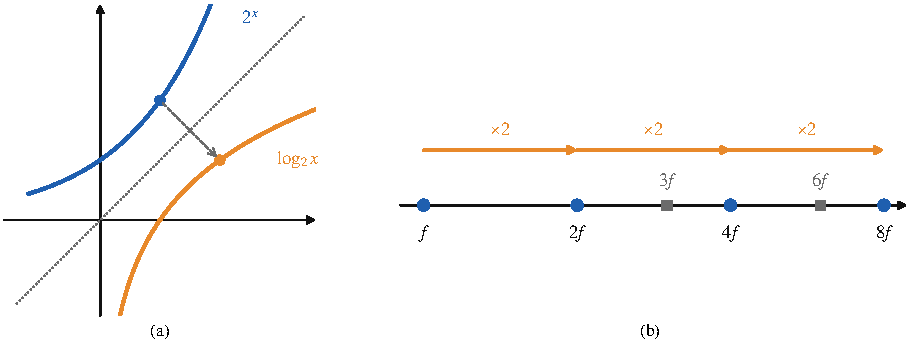
\includegraphics[width=0.8\linewidth]{figures/os-log.pdf}
\end{center}
{\footnotesize (a) Funkcje $2^x$ (niebieska) i $\log_2 x$ (pomarańczowa) są swoimi lustrzanymi odbiciami względem
prostej $y=x$ (kropkowana): odbicie punktu $(2,4)$ to $(4,2)$. (b) Na osi logarytmicznej kolejne podwojenia
$f,2f,4f,8f$ leżą w równych odstępach (pomarańczowe strzałki mają tę samą długość); punkty $3f$ i $6f$ też
dzieli dokładnie jeden taki krok, bo $\log_2 6-\log_2 3=1$.}\par\bigskip\hrule

\par\vspace{4mm}\noindent{\Large\bfseries Rysunek 1.4}\quad{\small(plik: rozdzial-01.tex)}\par\smallskip
\begin{center}

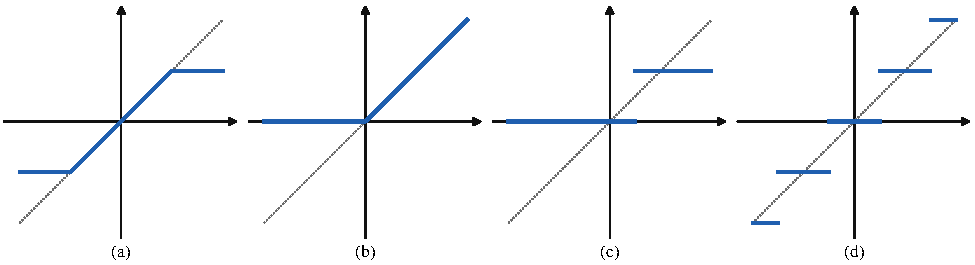
\includegraphics[width=0.8\linewidth]{figures/funkcje-pomocnicze.pdf}
\end{center}
{\footnotesize Cztery proste funkcje jednej zmiennej na tle prostej $y=x$ (kropkowana). (a) $\clip(x,-1,1)$ przycina wartości do przedziału.
(b) $\max(0,x)$, czyli $\ReLU$, zeruje wartości ujemne. (c) Wskaźnik $\indic{x\ge\frac12}$ jest równy $1$ albo $0$. (d) $\round(x)$ zaokrągla do najbliższej całkowitej.
Funkcje (c) i (d) mają skoki, więc nie da się ich używać w uczeniu przez gradient; dlatego dekoder w rozdziale~\ref{rozdz:dekoder} jest poza siecią.}\par\bigskip\hrule
\clearpage
\par\vspace{4mm}\noindent{\Large\bfseries Rysunek 2.1}\quad{\small(plik: rozdzial-02.tex)}\par\smallskip
\begin{center}

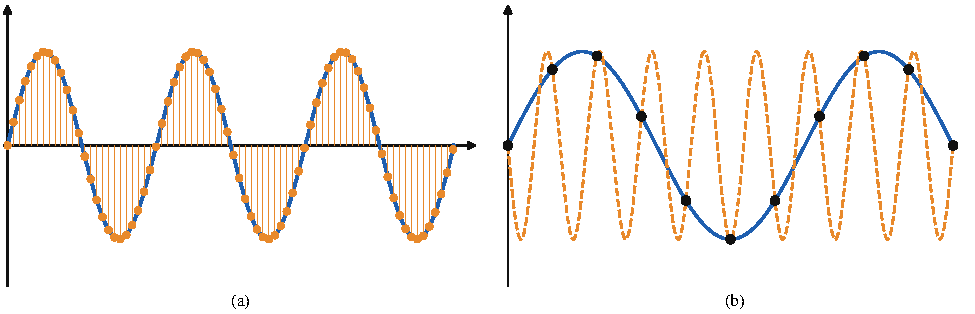
\includegraphics[width=0.8\linewidth]{figures/probkowanie.pdf}
\end{center}
{\footnotesize (a) Sinusoida $440\Hz$ (niebieska) i jej próbki przy $f_s=11\,025\Hz$ (pomarańczowe kropki): około
25 próbek na okres. (b) Aliasing: niebieska sinusoida $0{,}15f_s$ i pomarańczowa przerywana $-\sin$ o częstotliwości
$0{,}85 f_s$ przechodzą przez te same punkty (czarne kropki), więc po spróbkowaniu nie da się ich rozróżnić.}\par\bigskip\hrule

\par\vspace{4mm}\noindent{\Large\bfseries Rysunek 2.2}\quad{\small(plik: rozdzial-02.tex)}\par\smallskip
\begin{center}

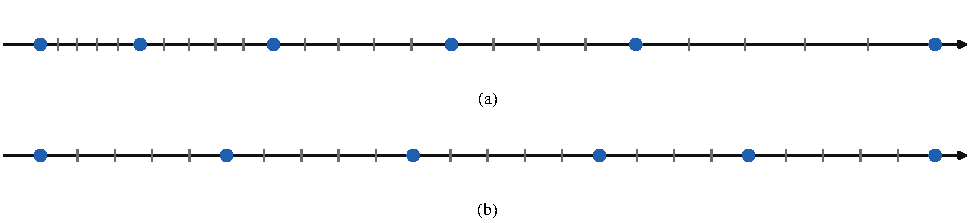
\includegraphics[width=0.8\linewidth]{figures/polsl-osie.pdf}
\end{center}
{\footnotesize Nuty od E2 do E4 (kreski) i sześć strun (niebieskie kropki). (a) Na osi liniowej częstotliwości
odstępy między półtonami rosną: ostatni jest ok.\ 3,8 raza większy niż pierwszy ($2^{23/12}$), więc niskie nuty
tłoczą się przy zerze. (b) Na osi $\log_2 f$ wszystkie półtony są równo oddalone o $1/12$ (z tw.~\ref{tw:log-iloczynu}).
Dlatego model liczy bliskość nut w półtonach, a nie w hercach.}\par\bigskip\hrule
\clearpage
\par\vspace{4mm}\noindent{\Large\bfseries Rysunek 3.1}\quad{\small(plik: rozdzial-03.tex)}\par\smallskip
\begin{center}

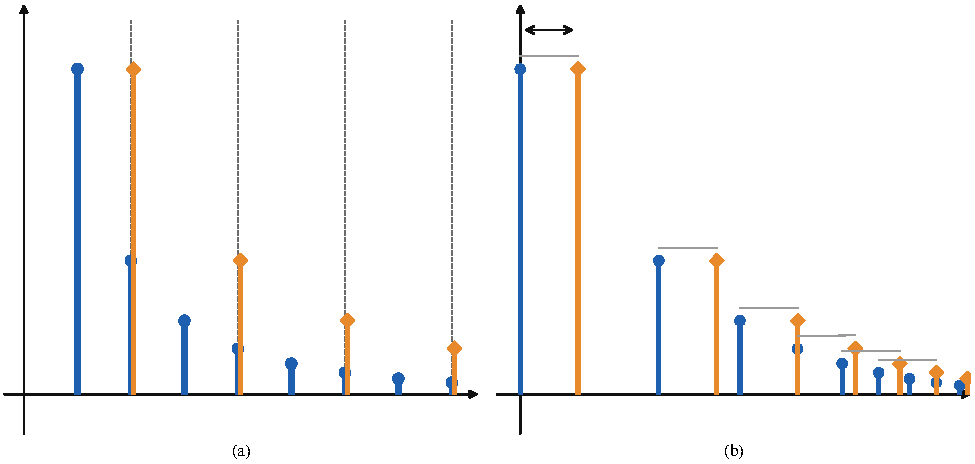
\includegraphics[width=0.8\linewidth]{figures/szereg-alikwotow.pdf}
\end{center}
{\footnotesize Widma szarpniętych strun liczone FFT. (a) Oś liniowa: prążki E2 (niebieskie) i E3 (pomarańczowe, nieco
przesunięte w prawo, żeby były widoczne). Każdy prążek E3 pada na parzysty prążek E2 (tw.~\ref{tw:oktawa-alik}).
(b) Oś w półtonach $12\log_2(f/f_{E2})$: wzorzec prążków E2 (niebieskie) i A2 (pomarańczowe) to ta sama figura
przesunięta o 5 półtonów (strzałka); kształt zależy tylko od numeru alikwotu, nie od wysokości.}\par\bigskip\hrule

\par\vspace{4mm}\noindent{\Large\bfseries Rysunek 3.2}\quad{\small(plik: rozdzial-03.tex)}\par\smallskip
\begin{center}

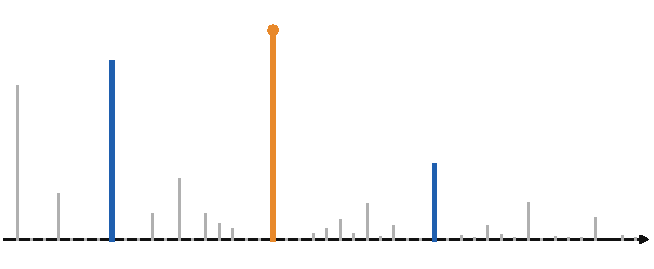
\includegraphics[width=0.8\linewidth]{figures/salience.pdf}
\end{center}
{\footnotesize Salience (suma energii sześciu pierwszych alikwotów) dla szarpniętej struny E3 ($m=52$) w funkcji numeru
kandydata $m$. Prawdziwa nuta (pomarańczowa) ma najwyższy słupek, ale kandydat o oktawę niżej ($m=40$, niebieski) jest
niewiele niższy, a ten o oktawę wyżej ($m=64$) też wyraźnie się wyróżnia. Wszystkie wartości liczone z widma FFT jednej nuty.}\par\bigskip\hrule
\clearpage
\par\vspace{4mm}\noindent{\Large\bfseries Rysunek 4.1}\quad{\small(plik: rozdzial-04.tex)}\par\smallskip
\begin{center}

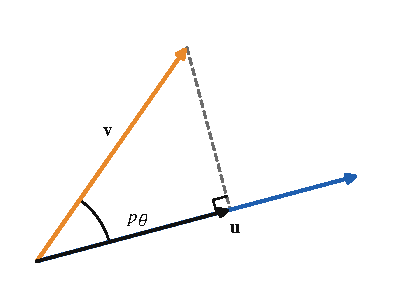
\includegraphics[width=0.8\linewidth]{figures/rzut.pdf}
\end{center}
{\footnotesize Rozkład z dowodu tw.~\ref{tw:cs}. Wektor $\vect v$ (pomarańczowy) rzutujemy na kierunek $\vect u$ (niebieski):
rzut $p$ (czarny) jest równoległy do $\vect u$, a odcinek kreskowany $\vect r=\vect v-\vect p$ jest do niego prostopadły (kąt prosty).
Długość rzutu to $\norm{\vect v}\cos\theta$, więc $\ip{\vect u}{\vect v}=\norm{\vect u}\norm{\vect v}\cos\theta$.}\par\bigskip\hrule

\par\vspace{4mm}\noindent{\Large\bfseries Rysunek 4.2}\quad{\small(plik: rozdzial-04.tex)}\par\smallskip
\begin{center}

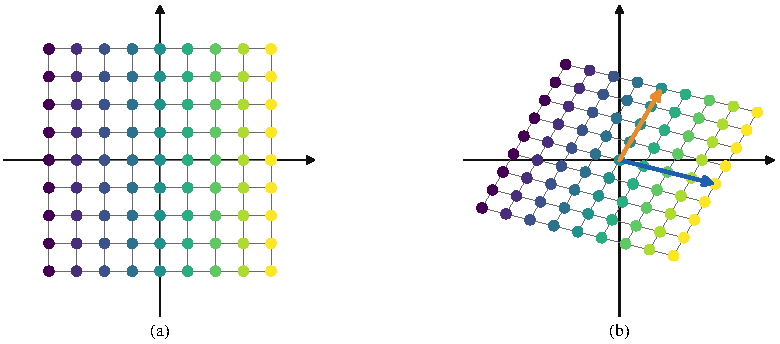
\includegraphics[width=0.8\linewidth]{figures/macierz-siatka.pdf}
\end{center}
{\footnotesize (a) Siatka punktów $9\times9$ w kwadracie $[-1,1]^2$, pokolorowana według współrzędnej $x$ (od fioletu do żółci).
(b) Obraz tej siatki po przekształceniu $\vect x\mapsto A\vect x$ z kolumnami $A\vect e_1$ (niebieska strzałka) i $A\vect e_2$
(pomarańczowa). Kolory pozwalają śledzić każdy punkt: proste zostają prostymi, a pole kwadratu rośnie $\abs{\det A}=1{,}2\cdot1{,}6+0{,}7\cdot0{,}4=2{,}2$ razy.}\par\bigskip\hrule
\clearpage
\par\vspace{4mm}\noindent{\Large\bfseries Rysunek 5.1}\quad{\small(plik: rozdzial-05.tex)}\par\smallskip
\begin{center}

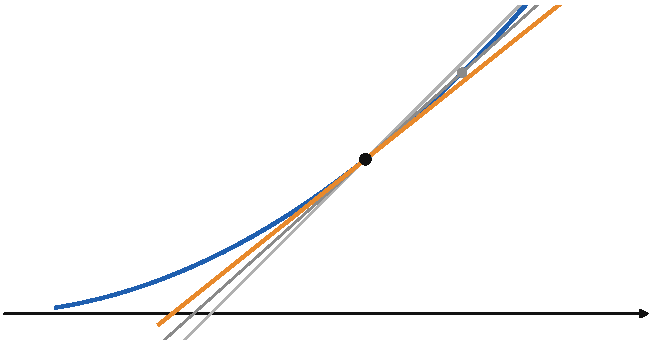
\includegraphics[width=0.8\linewidth]{figures/sieczne.pdf}
\end{center}
{\footnotesize Pochodna jako granica nachyleń. Funkcja $x^2$ (niebieska) i sieczne (szare) przez punkt $(3,9)$ (czarny) i punkty
oddalone o $h=1{,}5$ oraz $0{,}75$. Gdy $h\to0$, sieczna dąży do stycznej (pomarańczowa) o nachyleniu $f'(3)=6$.}\par\bigskip\hrule

\par\vspace{4mm}\noindent{\Large\bfseries Rysunek 5.2}\quad{\small(plik: rozdzial-05.tex)}\par\smallskip
\begin{center}

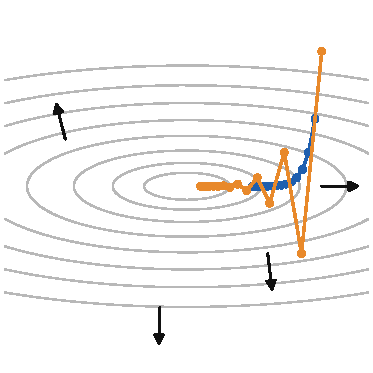
\includegraphics[width=0.8\linewidth]{figures/spadek.pdf}
\end{center}
{\footnotesize Spadek gradientu dla $L=\tfrac12(x^2+10y^2)$ (szare warstwice) z punktu $(1,1)$. Czarne strzałki to gradient w kilku punktach:
zawsze prostopadły do warstwicy i skierowany pod górę, więc krok idzie w przeciwną stronę. Niebieska ścieżka ($\eta=0{,}05$, 14 kroków)
schodzi gładko, ale wolno; pomarańczowa ($\eta=0{,}15$) przeskakuje przez dolinę i zygzakuje. Obie obliczone programem.}\par\bigskip\hrule
\clearpage
\par\vspace{4mm}\noindent{\Large\bfseries Rysunek 6.1}\quad{\small(plik: rozdzial-06.tex)}\par\smallskip
\begin{center}

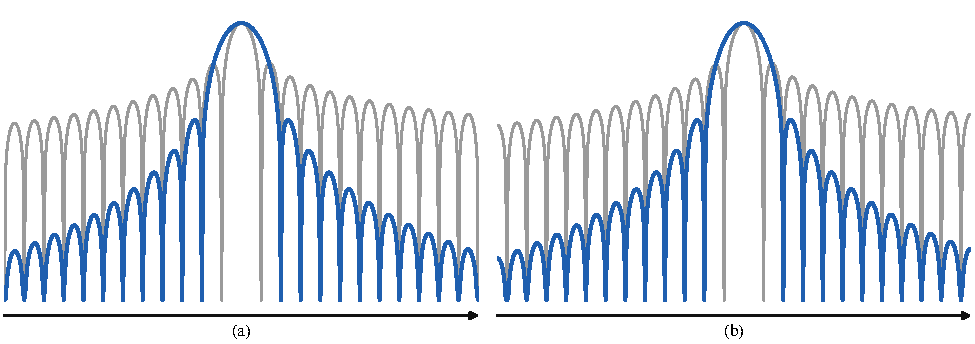
\includegraphics[width=0.8\linewidth]{figures/przeciek.pdf}
\end{center}
{\footnotesize Widmo (w decybelach, skala pionowa wspólna, od $-90$ do $0\dB$) tonu z $N=128$ próbek. (a) Ton dokładnie w prążku: okno
prostokątne (szare) daje wąski pik, ale ze słabo opadającymi listkami (pierwszy $-13\dB$); okno Hanna (niebieskie) ma szerszy pik i listki o ok.\ $18\dB$ niższe.
(b) Ton w połowie między prążkami: pik jest niższy, a listki prostokątnego okna jeszcze wyższe względem Hanna.}\par\bigskip\hrule

\par\vspace{4mm}\noindent{\Large\bfseries Rysunek 6.2}\quad{\small(plik: rozdzial-06.tex)}\par\smallskip
\begin{center}

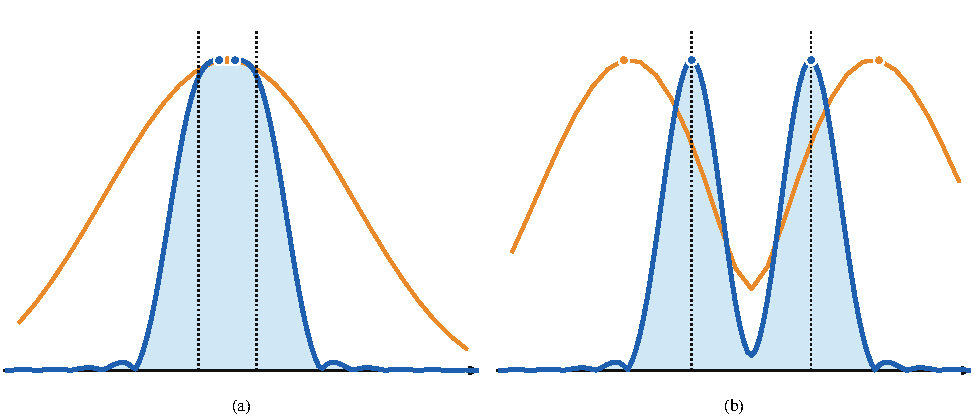
\includegraphics[width=0.8\linewidth]{figures/rozdzielczosc.pdf}
\end{center}
{\footnotesize Widmo (okno Hanna) sumy dwóch sinusoid z oknem $N=4096$ (niebieskie) i $N=1024$ (pomarańczowe); kropkowane pionowe linie to prawdziwe częstotliwości.
(a) E2 i F2 (półton, $4{,}9\Hz$): długie okno daje dwa bliskie piki w złych miejscach (interferencja), krótkie jeden szeroki pagórek. (b) E2 i F\#2 ($10{,}1\Hz$): długie okno rozdziela dwa
tony prawie bez błędu położenia, krótkie daje dwa piki odsunięte od prawdy o kilka herców. Dlatego model dostaje dwa okna --- długie dla wysokości, krótkie dla czasu --- i uczy się łączyć wskazówki z wielu klatek.}\par\bigskip\hrule
\clearpage
\par\vspace{4mm}\noindent{\Large\bfseries Rysunek 7.1}\quad{\small(plik: rozdzial-07.tex)}\par\smallskip
\begin{center}

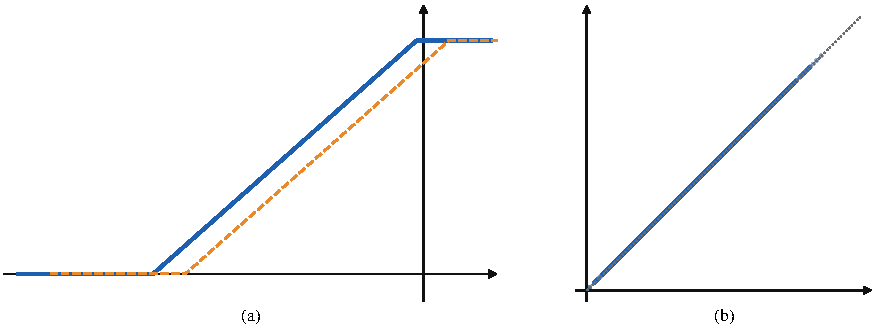
\includegraphics[width=0.8\linewidth]{figures/niezmiennik-glosnosci.pdf}
\end{center}
{\footnotesize (a) Cecha jako funkcja $\log_{10}A$ (niebieska): płaski początek (cisza poniżej $60\dB$ od referencji), liniowy wzrost i przycięcie na $1{,}3$.
Nagranie 3 razy głośniejsze (pomarańczowa przerywana) ma tę samą krzywą, bo referencja przesuwa się razem z poziomami (tw.~\ref{tw:glosnosc}).
(b) Wartości cech tego samego nagrania (poziomo) i nagrania 10 razy cichszego (pion): wszystkie punkty leżą na przekątnej (kropkowana).}\par\bigskip\hrule

\par\vspace{4mm}\noindent{\Large\bfseries Rysunek 7.2}\quad{\small(plik: rozdzial-07.tex)}\par\smallskip
\begin{center}

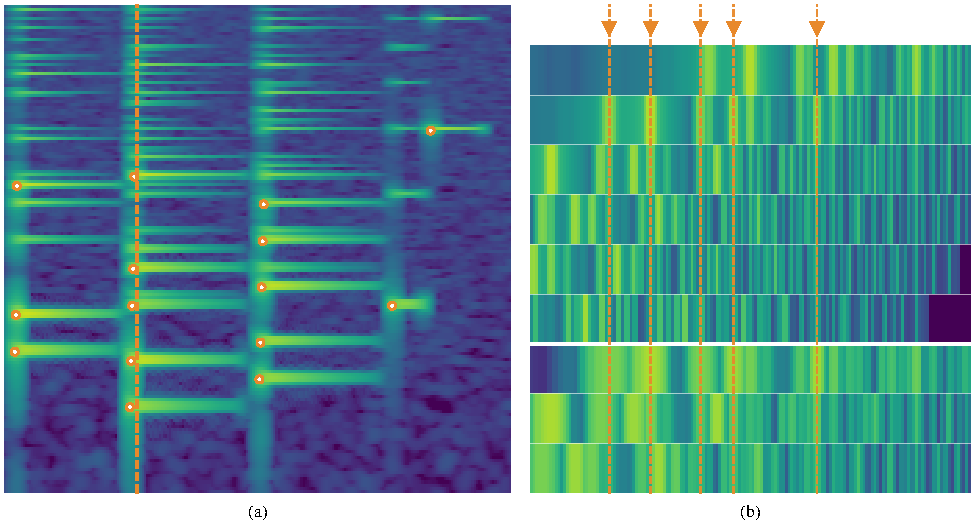
\includegraphics[width=0.8\linewidth]{figures/hcqt-przyklad.pdf}
\end{center}
{\footnotesize HCQT syntetycznego, 6-sekundowego nagrania gitary. (a) Kanał $h=1$: czas poziomo (243 klatki), wysokość pionowo (159 binów); jasne ślady to alikwoty
grających nut, kółka z pomarańczowym brzegiem to początki prawdziwych nut, przerywana linia to klatka pokazana w (b). (b) Cała jedna klatka: 9 kanałów (wiersze) $\times$ 159 binów (kolumny).
Pomarańczowe trójkąty wskazują prawdziwe nuty: pod każdym z nich w kolumnie pojawiają się jasne plamy w wielu kanałach naraz, bo alikwoty kandydata ustawiono w jednej kolumnie.}\par\bigskip\hrule
\clearpage
\par\vspace{4mm}\noindent{\Large\bfseries Rysunek 8.1}\quad{\small(plik: rozdzial-08.tex)}\par\smallskip
\begin{center}

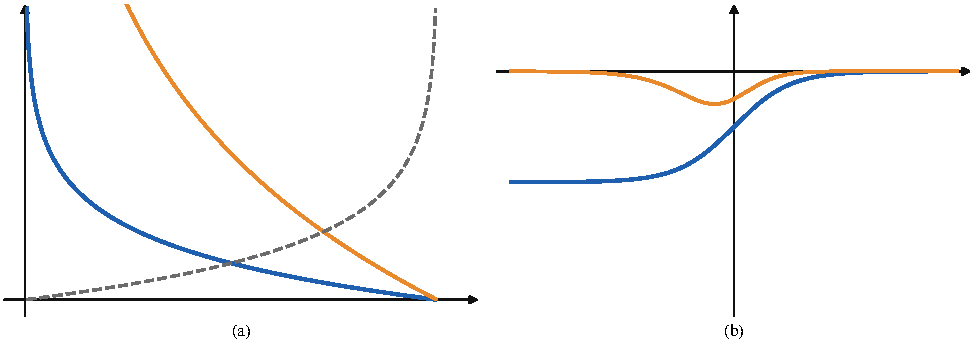
\includegraphics[width=0.8\linewidth]{figures/bce.pdf}
\end{center}
{\footnotesize (a) Strata BCE w funkcji $p$: dla $y=1$ ($-\ln p$, niebieska) i z wagą $\alpha=4$ (pomarańczowa) rośnie do nieskończoności, gdy $p\to0$; dla $y=0$ ($-\ln(1-p)$, szara przerywana)
rośnie, gdy $p\to1$. (b) Gradient po logicie dla $y=1$: BCE (niebieska, $\sigma-1$) pozostaje blisko $-1$ przy dużym błędzie; gradient błędu kwadratowego (pomarańczowa) zanika w nasyceniu.}\par\bigskip\hrule

\par\vspace{4mm}\noindent{\Large\bfseries Rysunek 8.2}\quad{\small(plik: rozdzial-08.tex)}\par\smallskip
\begin{center}

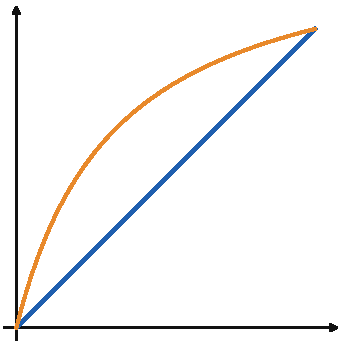
\includegraphics[width=0.8\linewidth]{figures/kalibracja.pdf}
\end{center}
{\footnotesize Optymalne prawdopodobieństwo $p^\ast$ (pion) w zależności od prawdziwej częstości $q$ (poziom) dla wagi $\alpha=1$ (niebieska, leży na przekątnej) i $\alpha=4$ (pomarańczowa, nad przekątną). Waga klasy dodatniej
przesuwa wyjścia sieci w górę; dekoder (rozdział~\ref{rozdz:dekoder}) musi to uwzględnić przez progi dobrane na walidacji.}\par\bigskip\hrule
\clearpage
\par\vspace{4mm}\noindent{\Large\bfseries Rysunek 9.1}\quad{\small(plik: rozdzial-09.tex)}\par\smallskip
\begin{center}

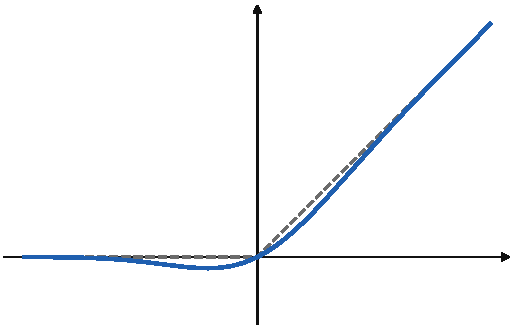
\includegraphics[width=0.8\linewidth]{figures/gelu.pdf}
\end{center}
{\footnotesize GELU (niebieska) i ReLU (szara przerywana). GELU jest gładką wersją ReLU: w odróżnieniu od niego ma niewielką ujemną „zatokę” (minimum ok.\ $-0{,}17$) i nie ma ostrego załamania w zerze,
więc ma pochodną wszędzie.}\par\bigskip\hrule

\par\vspace{4mm}\noindent{\Large\bfseries Rysunek 9.2}\quad{\small(plik: rozdzial-09.tex)}\par\smallskip
\begin{center}

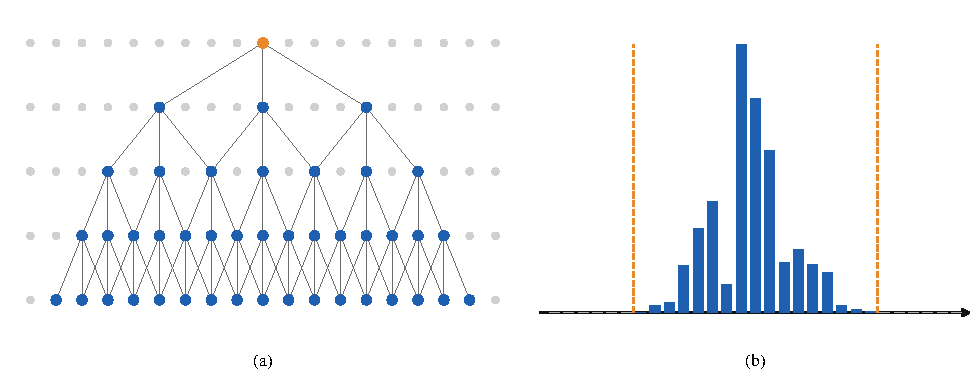
\includegraphics[width=0.8\linewidth]{figures/pole-widzenia.pdf}
\end{center}
{\footnotesize (a) Schemat czterech konwolucji czasowych z jądrem $3$ i dylatacjami $1$ (trzon), $1,2,4$ (od wejścia na dole do wyjścia na górze): pomarańczowa kropka to jedna klatka wyjścia, niebieskie to klatki wejścia, od których zależy
(zasięg $\pm8=1+1+2+4$). Z dylatacją pole widzenia rośnie wykładniczo, a nie liniowo, przy tej samej liczbie parametrów.
(b) Pomiar: moduł gradientu jednej wartości wyjścia po wejściu w funkcji odległości w klatkach dla stosu z trzonem $3\times7$ i trzema blokami z dylatacjami $1,2,4$ (losowe wagi, PyTorch): gradient jest niezerowy dokładnie dla $|t|\le8=1+(1+2+4)$ (niebieskie) i zerowy poza (szare).}\par\bigskip\hrule
\clearpage
\par\vspace{4mm}\noindent{\Large\bfseries Rysunek 9.3}\quad{\small(plik: rozdzial-09.tex)}\par\smallskip
\begin{center}

\begin{tikzpicture}[>=Stealth,node distance=6mm]
  \node[blok,minimum width=14mm] (x) {$\vect x$};
  \node[blok,minimum width=16mm,right=of x] (ln) {$\LN$};
  \node[blok,minimum width=16mm,right=of ln] (f) {$F$};
  \node[blok,minimum width=14mm,right=of f] (drop) {$\Drop$};
  \node[wezel,right=8mm of drop] (plus) {$+$};
  \node[right=7mm of plus] (y) {$\vect y$};
  \draw[wektor] (x)--(ln); \draw[wektor] (ln)--(f); \draw[wektor] (f)--(drop); \draw[wektor] (drop)--(plus); \draw[wektor] (plus)--(y);
  \draw[wektor] (x.north) -- ++(0,6mm) -| (plus.north);
\end{tikzpicture}
\end{center}
{\footnotesize Blok resztkowy typu „pre-norm”, jak w warstwach Gen~6: wejście $\vect x$ jest normalizowane (LN), przechodzi przez $F$ (konwolucja albo uwaga) i dropout, a następnie dodawane do niezmienionego $\vect x$ (górna ścieżka). Wynik: $\vect y=\vect x+\Drop(F(\LN(\vect x)))$.}\par\bigskip\hrule

\par\vspace{4mm}\noindent{\Large\bfseries Rysunek 10.1}\quad{\small(plik: rozdzial-10.tex)}\par\smallskip
\begin{center}

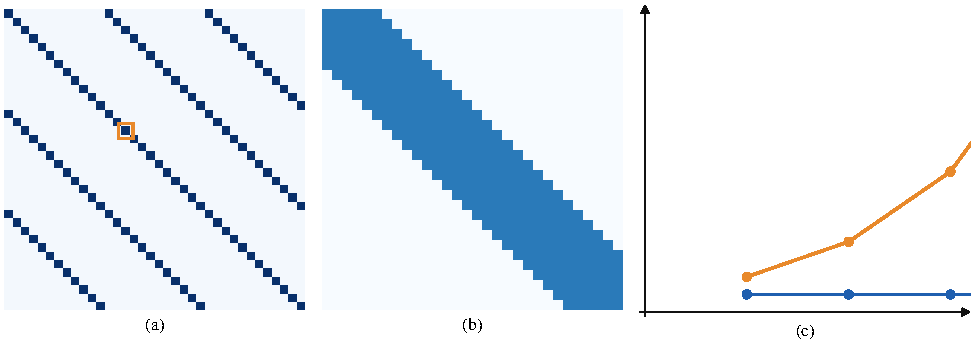
\includegraphics[width=0.8\linewidth]{figures/uwaga.pdf}
\end{center}
{\footnotesize (a) Zabawka: $36$ półtonów, a zapytanie i klucz to wskazanie klasy wysokości $(i\bmod12)$. Każdy wiersz macierzy wag $\alpha$ ma ciemne pola tylko dla tej samej klasy, czyli co $12$ półtonów: wysokość $14$ (pomarańczowa ramka)
patrzy na $2$, $14$ i $26$ --- uwaga potrafi „zobaczyć” oktawy. (b) Maska okna $\abs{t-u}\le5$ dla $30$ klatek: tylko pasmo wokół przekątnej ma niezerowe wagi. (c) Odchylenie standardowe $\ip{\vect q}{\vect k}$ dla wymiarów $d=4,16,64,256$ (oś pozioma $\log_2d$):
bez skalowania (pomarańczowa) rośnie jak $\sqrt d$, po podzieleniu przez $\sqrt d$ (niebieska) jest równe $1$. Obliczone z $10^5$ losowych par.}\par\bigskip\hrule
\clearpage
\par\vspace{4mm}\noindent{\Large\bfseries Rysunek 10.2}\quad{\small(plik: rozdzial-10.tex)}\par\smallskip
\begin{center}

\begin{tikzpicture}[>=Stealth,node distance=5mm,font=\small]
  \node[blok,minimum width=9mm] (h) {$H$};
  \node[blok,above right=2mm and 9mm of h,minimum width=9mm] (q) {$Q$};
  \node[blok,right=9mm of h,minimum width=9mm] (k) {$K$};
  \node[blok,below right=2mm and 9mm of h,minimum width=9mm] (v) {$V$};
  \node[blok,right=9mm of k,minimum width=16mm] (s) {$\softmax\!\big(\tfrac{QK^\top}{\sqrt d}+B\big)$};
  \node[blok,right=9mm of s,minimum width=9mm] (o) {$\times V$};
  \draw[wektor] (h)--(q); \draw[wektor] (h)--(k); \draw[wektor] (h)--(v);
  \draw[wektor] (q.east)--++(2mm,0)|-(s.west); \draw[wektor] (k)--(s);
  \draw[wektor] (s)--(o); \draw[wektor] (v.east)--++(2mm,0) -| ([xshift=3mm]o.south);
\end{tikzpicture}
\end{center}
{\footnotesize Przepływ danych jednej głowicy uwagi. Wektory cech $H\in\R^{n\times D}$ są rzutowane na $Q,K,V\in\R^{n\times d_h}$; iloczyny $QK^\top\in\R^{n\times n}$ (wyniki dopasowania), dzielone przez $\sqrt{d}$ i powiększone o premie $B$, przechodzą przez softmax
wiersz po wierszu; powstałe wagi mnożą $V$ i dają wyjście $n\times d_h$.}\par\bigskip\hrule

\par\vspace{4mm}\noindent{\Large\bfseries Rysunek 11.1}\quad{\small(plik: rozdzial-11.tex)}\par\smallskip
\begin{center}

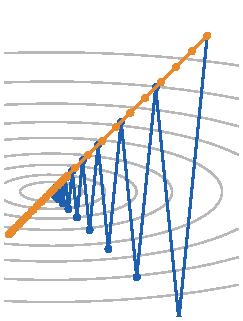
\includegraphics[width=0.8\linewidth]{figures/adam-dolina.pdf}
\end{center}
{\footnotesize Ta sama dolina $L=\frac12(x^2+10y^2)$ co w rozdziale~\ref{rozdz:pochodne}, start $(1,1)$, $40$ kroków. Niebieska: spadek gradientu z optymalnym krokiem $2/11$ (strata końcowa $6\cdot10^{-7}$).
Pomarańczowa: Adam z $\eta=0{,}1$ (strata końcowa $0{,}056$: długie kroki w obu osiach, ale potem drży wokół minimum). Szare warstwice to poziomy strat. Na tej prostej paraboli, przy idealnie dobranym kroku, wygrywa zwykły spadek gradientu. Obie ścieżki obliczone programem.}\par\bigskip\hrule
\clearpage
\par\vspace{4mm}\noindent{\Large\bfseries Rysunek 11.2}\quad{\small(plik: rozdzial-11.tex)}\par\smallskip
\begin{center}

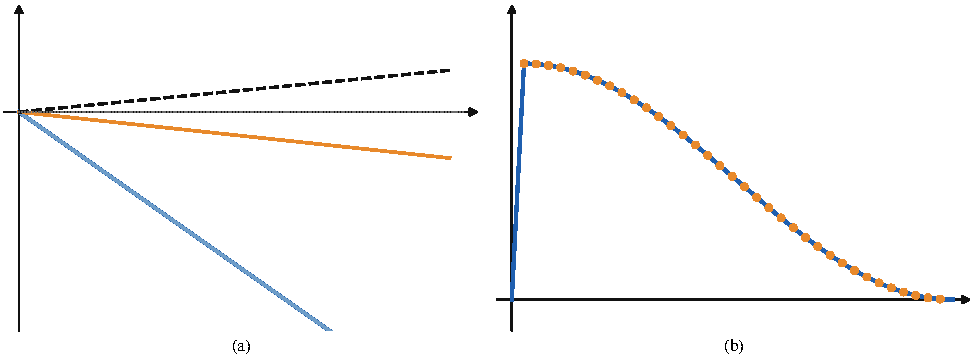
\includegraphics[width=0.8\linewidth]{figures/optymalizacja.pdf}
\end{center}
{\footnotesize (a) Spadek gradientu dla $\lambda=10$ ($\log_{10}|x|$ w kolejnych krokach): $\eta=0{,}05$ (niebieska) i $0{,}15$ (jasnoniebieska) zbiegają; $\eta=0{,}19$ (pomarańczowa) zbiega z wolno gasnącym drżeniem; $\eta=0{,}21>2/\lambda$ (czarna przerywana) rozbiega się. Szara kropkowana to poziom początkowy.
(b) Harmonogram kroku z rozgrzewką i spadkiem kosinusowym (niebieska) oraz wartości zapisane w dzienniku prawdziwego uczenia Gen~6 po każdej epoce (pomarańczowe kropki): leżą dokładnie na krzywej.}\par\bigskip\hrule

\par\vspace{4mm}\noindent{\Large\bfseries Rysunek 12.1}\quad{\small(plik: rozdzial-12.tex)}\par\smallskip
\begin{center}

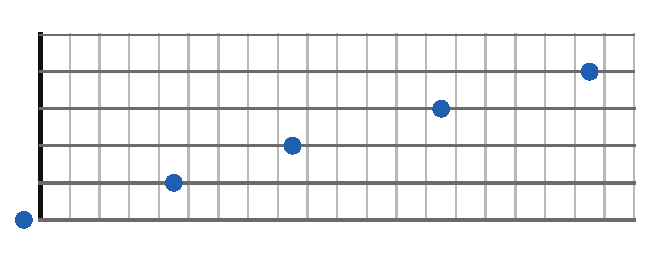
\includegraphics[width=0.8\linewidth]{figures/gryf-e4.pdf}
\end{center}
{\footnotesize Gryf z $20$ progami; struny od najcieńszej (góra) do najgrubszej (dół). Niebieskie kropki to wszystkie pięć pozycji nuty E4: próg~0 (struna pusta, kropka przed siodełkiem), $5$, $9$, $14$ i $19$. Wysokość nie wystarcza do ustalenia pozycji;
o strunie decyduje barwa dźwięku (struny o różnej grubości mają inny rozkład alikwotów) i kontekst muzyczny.}\par\bigskip\hrule
\clearpage
\par\vspace{4mm}\noindent{\Large\bfseries Rysunek 12.2}\quad{\small(plik: rozdzial-12.tex)}\par\smallskip
\begin{center}

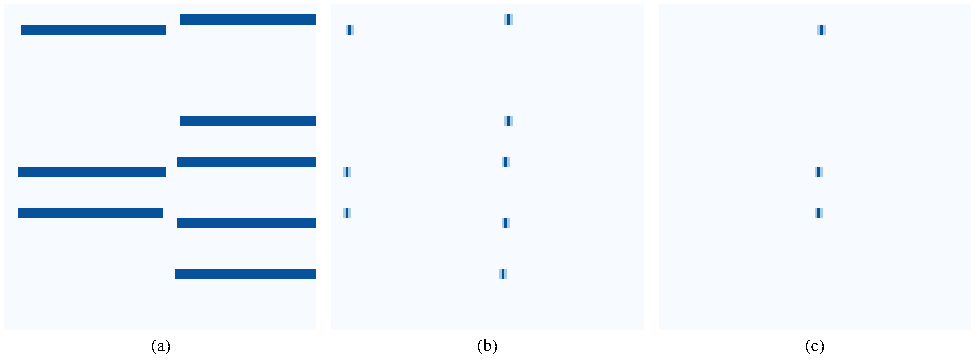
\includegraphics[width=0.8\linewidth]{figures/mapy-celow.pdf}
\end{center}
{\footnotesize Mapy celów syntetycznego nagrania z $15$ nutami (fragment: $110$ klatek, półtony $4$--$35$): (a) „brzmi” --- poziome kreski trwających nut, (b) początki --- pojedyncze kropki (jasne punkty to $1$, ich pionowe sąsiedztwo w czasie to miękkie $0{,}4$), (c) końce.
Mapy początków i końców są rzadkie: tylko $0{,}12\%$ komórek początków jest równa $1$ (rozdział~\ref{rozdz:strata}). Mapy zbudowane kodem z repozytorium.}\par\bigskip\hrule

\par\vspace{4mm}\noindent{\Large\bfseries Rysunek 13.1}\quad{\small(plik: rozdzial-13.tex)}\par\smallskip
\begin{center}

\begin{tikzpicture}[>=Stealth,x=1cm,y=1cm,font=\small]
  \tikzset{b/.style={blok,minimum height=11mm,minimum width=24mm,font=\small,text width=24mm,align=center},
           kszt/.style={font=\footnotesize,text=black!70}}
  \node[b] (x) at (0,0) {HCQT};
  \node[b,right=8mm of x] (stem) {trzon\\conv $3{\times}7$};
  \node[b,right=8mm of stem,fill=blue!8!white] (hb) {$3\times$ blok harmoniczny};
  \node[b,right=8mm of hb] (dw) {zejście do półtonów\\conv $1{\times}3$, krok $3$\\$+\,e_s$};
  \draw[wektor] (x)--(stem); \draw[wektor] (stem)--(hb); \draw[wektor] (hb)--(dw);
  \node[kszt,below=1mm of x] {$[B,9,T,159]$};
  \node[kszt,below=1mm of stem] {$[B,48,T,159]$};
  \node[kszt,below=1mm of hb] {$[B,48,T,159]$};
  \node[kszt,below=1mm of dw] {$[B,T,53,64]$};
  \node[b,below=17mm of x,fill=orange!10!white] (ctx) {$2\times$ warstwa kontekstu\\(uwaga w czasie\\+ uwaga między wysokościami\\+ FF)};
  \node[b,right=8mm of ctx] (ln) {LayerNorm};
  \node[b,right=8mm of ln,fill=green!8!white] (heads) {głowice:\\początek, brzmi, koniec,\\głośność, tabulatura};
  \draw[wektor] (dw.south) -- ++(0,-9mm) -| (ctx.north);
  \draw[wektor] (ctx)--(ln); \draw[wektor] (ln)--(heads);
  \node[kszt,below=1mm of ctx] {$[B,T,53,64]$};
  \node[kszt,below=1mm of ln] {$[B,T,53,64]$};
  \node[kszt,below=1mm of heads] {$[B,T,53]\ \times4,\ [B,T,6,21]$};
\end{tikzpicture}
\end{center}
{\footnotesize Przepływ tensorów w Gen~6 ($B$ --- liczba nagrań w paczce, $T$ --- liczba klatek). Pierwsza połowa (rozdz.~\ref{rozdz:architektura}, niebieskie pole): cechy HCQT przechodzą przez trzon i trzy bloki harmoniczne,
a potem „schodzą” z $159$ binów do $53$ półtonów ($64$ liczby opisu na każdą parę klatka--półton). Druga połowa (rozdz.~\ref{rozdz:uwaga-wys}): dwie warstwy kontekstu (pomarańczowe pole), normalizacja i pięć głowic (zielone pole). Łącznie $249\,219$ parametrów.}\par\bigskip\hrule
\clearpage
\par\vspace{4mm}\noindent{\Large\bfseries Rysunek 13.2}\quad{\small(plik: rozdzial-13.tex)}\par\smallskip
\begin{center}

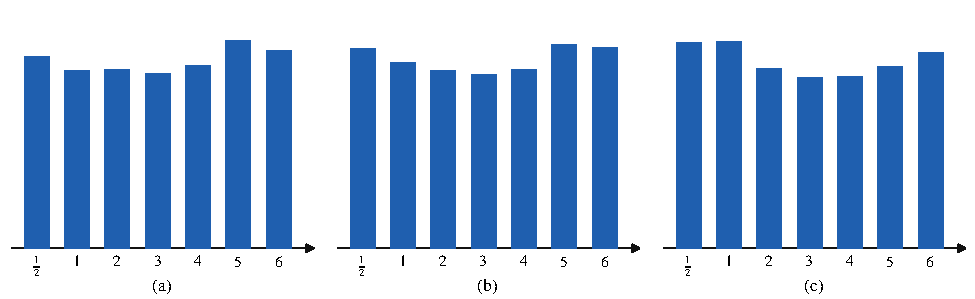
\includegraphics[width=0.8\linewidth]{figures/harm-wagi.pdf}
\end{center}
{\footnotesize Średnie wartości bezwzględne wag $W_h$ w grupach wejść odpowiadających alikwotom $h=\tfrac12,1,2,3,4,5,6$ (pod słupkami) dla trzech bloków (a), (b), (c) prawdziwego, wytrenowanego modelu Gen~6 (skala pionowa wspólna, od zera).
Wszystkie siedem miejsc ma wagi podobnej wielkości ($0{,}088$--$0{,}107$): żadne nie zostało „wyłączone”. Wielkość wag nie dowodzi jednak ważności (brak badania ablacyjnego, zob.\ rozdział~\ref{rozdz:wyniki}).}\par\bigskip\hrule

\par\vspace{4mm}\noindent{\Large\bfseries Rysunek 14.1}\quad{\small(plik: rozdzial-14.tex)}\par\smallskip
\begin{center}

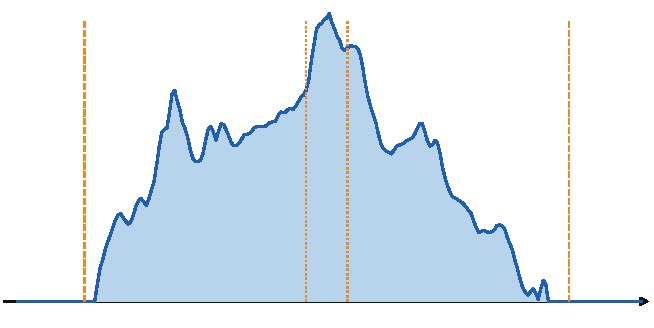
\includegraphics[width=0.8\linewidth]{figures/pole-widzenia-modelu.pdf}
\end{center}
{\footnotesize Pomiar pola widzenia prawdziwego modelu Gen~6: $\log_{10}$ modułu gradientu logitu początku w klatce $t$ (jeden półton) po cechach wejściowych w klatce $t+\Delta t$, od $-125$ do $125$ klatek (pomarańczowe pionowe: kropkowane $\pm8$ --- zasięg samej części konwolucyjnej,
przerywane $\pm94$ --- zasięg całej sieci). Poza $\pm94$ zależności nie ma (wypełnienie opada do dna skali); wewnątrz maleje o kilka rzędów wielkości.}\par\bigskip\hrule
\clearpage
\par\vspace{4mm}\noindent{\Large\bfseries Rysunek 14.2}\quad{\small(plik: rozdzial-14.tex)}\par\smallskip
\begin{center}

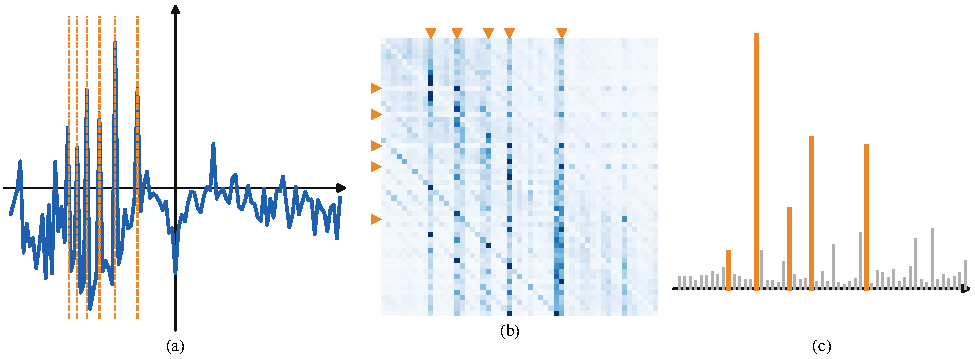
\includegraphics[width=0.8\linewidth]{figures/uwaga-wysokosci.pdf}
\end{center}
{\footnotesize Uwaga między wysokościami w prawdziwym modelu Gen~6 (warstwa kontekstu 0). (a) Wyuczona premia $r_d$ głowicy $2$: niebieska krzywa, pomarańczowe przerywane linie to odległości $-12\log_2h$ dla $h=2,\dots,7$ ($-12,-19,-24,-28,-31,-34$). Dokładnie siedem odległości ma premię powyżej $0{,}6$:
sześć z nich to te interwały alikwotów, a siódma to $+12$. (b) Macierz wag uwagi (średnia z czterech głowic; wiersz --- zapytanie, kolumna --- klucz) w klatce nagrania, w której gra $5$ nut (pomarańczowe znaczniki przy osiach to ich półtony). (c) Wiersz najniższej nuty ($m=45$):
pomarańczowe słupki to pozostałe nuty akordu; trafia w nie $45\%$ całej wagi, podczas gdy równomierny rozkład dałby $4/53=7{,}5\%$.}\par\bigskip\hrule

\par\vspace{4mm}\noindent{\Large\bfseries Rysunek 15.1}\quad{\small(plik: rozdzial-15.tex)}\par\smallskip
\begin{center}

\begin{tikzpicture}[>=Stealth,font=\small]
  \tikzset{b/.style={blok,text width=21mm,minimum height=13mm,align=center,font=\footnotesize}}
  \node[b] (zr) {źródła:\\klasyka $0{,}5$\\GuitarSet $0{,}3$\\środowiska $0{,}2$};
  \node[b,right=6mm of zr] (wy) {$16$ wycinków\\po $192$ klatki};
  \node[b,right=6mm of wy] (au) {augmentacje\\(tab.~\ref{tab:augmentacje})};
  \node[b,right=6mm of au,fill=blue!8!white] (si) {sieć Gen~6\\$249\,219$ param.};
  \node[b,right=6mm of si] (st) {$5$ strat\\$\times$ maski $a_g$};
  \node[b,right=6mm of st,fill=orange!10!white] (op) {$\mathcal L$, gradient,\\przycięcie $\le1$,\\AdamW};
  \draw[wektor] (zr)--(wy); \draw[wektor] (wy)--(au); \draw[wektor] (au)--(si); \draw[wektor] (si)--(st); \draw[wektor] (st)--(op);
  \draw[wektor] (op.south) -- ++(0,-6mm) -| node[pos=0.25,below,font=\footnotesize]{nowe wagi $\vect\theta$ ($\times1000$ w epoce)} (si.south);
\end{tikzpicture}
\end{center}
{\footnotesize Jeden krok uczenia Gen~6. Z trzech źródeł (wagi losowania w ramce) losuje się $16$ wycinków po $4{,}46$ s, zniekształca je augmentacjami, przepuszcza przez sieć, liczy pięć strat z maskami dostępności etykiet, sumuje je do $\mathcal L$, przycina gradient do normy $1$ i aktualizuje wagi optymalizatorem AdamW; po $1000$ takich krokach kończy się epoka.}\par\bigskip\hrule
\clearpage
\par\vspace{4mm}\noindent{\Large\bfseries Rysunek 15.2}\quad{\small(plik: rozdzial-15.tex)}\par\smallskip
\begin{center}

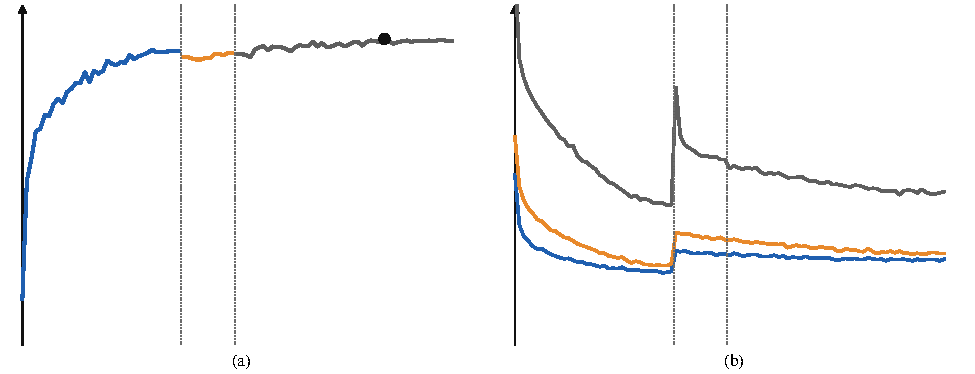
\includegraphics[width=0.8\linewidth]{figures/uczenie.pdf}
\end{center}
{\footnotesize Prawdziwy przebieg uczenia Gen~6 (dziennik \texttt{docs/wyniki/epoki.csv}, $97$ epok). (a) F1 nut na stałej próbie walidacyjnej $180$ nagrań (skala od $66$ do $93\%$): sesja~1 niebieska, sesja~3 pomarańczowa, sesja~4 ciemnoszara; czarna kropka to wybrana epoka $81$ ($90{,}27\%$). Pionowe linie rozdzielają sesje.
(b) $\log_{10}$ strat uczących: początki (niebieska), brzmi (pomarańczowa), tabulatura (ciemnoszara). Skok strat na początku sesji~3 i~4 to efekt restartu kroku i nowych, trudniejszych danych.}\par\bigskip\hrule

\par\vspace{4mm}\noindent{\Large\bfseries Rysunek 16.1}\quad{\small(plik: rozdzial-16.tex)}\par\smallskip
\begin{center}

\begin{tikzpicture}[>=Stealth,node distance=4.5mm,font=\footnotesize]
  \tikzset{st/.style={draw,rounded corners=2mm,thick,minimum height=8mm,minimum width=17mm,align=center,fill=white},
           eti/.style={font=\scriptsize,midway,fill=white,inner sep=1pt}}
  \node[st] (cisza) {cisza};
  \node[st,right=22mm of cisza,fill=blue!8!white] (gra) {nuta trwa};
  \node[st,right=22mm of gra] (kon) {zapis\\nuty};
  \draw[->,thick] (cisza) -- node[eti,above=1mm]{pik $p_\mathrm{on}$} (gra);
  \draw[->,thick] (gra) -- node[eti,above=1mm]{pik $p_\mathrm{off}$} node[eti,below=1mm]{lub \texttt{gap}$>g_\mathrm{max}$} (kon);
  \draw[->,thick] (kon.south) -- ++(0,-6mm) -| (cisza.south);
  \draw[->,thick] (gra.north) -- ++(0,5mm) -| node[eti,pos=0.25,above=1mm]{pik $p_\mathrm{on}$: ponowne szarpnięcie} (gra.north east);
\end{tikzpicture}
\end{center}
{\footnotesize Maszyna stanów dekodera dla jednego półtonu. Z ciszy wychodzi się na piku początku; nuta trwa, dopóki $p_\mathrm{fr}\ge\theta_\mathrm{fr}$; kończy ją pik końca albo przerwa dłuższa niż $g_\mathrm{max}$ klatek; nowy pik początku w trakcie nuty kończy ją i zaczyna następną.}\par\bigskip\hrule
\clearpage
\par\vspace{4mm}\noindent{\Large\bfseries Rysunek 16.2}\quad{\small(plik: rozdzial-16.tex)}\par\smallskip
\begin{center}

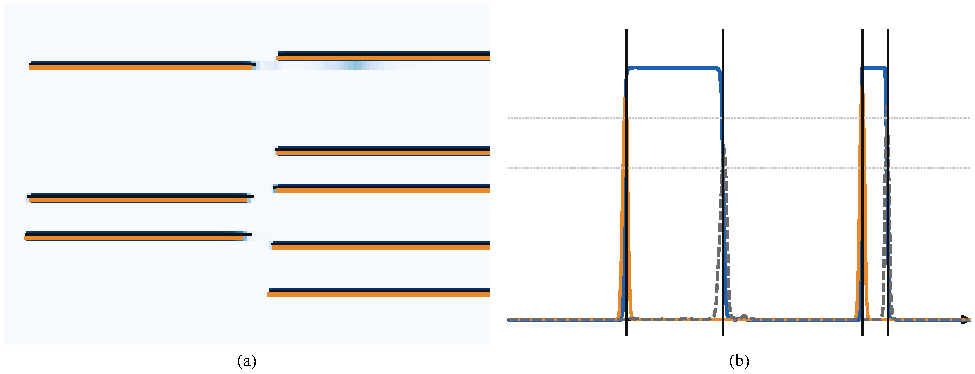
\includegraphics[width=0.8\linewidth]{figures/dekoder-model.pdf}
\end{center}
{\footnotesize Dekoder na wyjściach prawdziwego modelu Gen~6 (syntetyczne nagranie z $15$ nutami). (a) Mapa $p_\mathrm{fr}$ (jasność), fragment $110$ klatek i półtony $4$--$39$; czarne kreski --- prawdziwe nuty, pomarańczowe --- nuty z dekodera (każda para blisko siebie; największy błąd początku $18{,}7\ms$).
(b) Trzy głowice dla jednego półtonu z dwiema nutami: $p_\mathrm{fr}$ (niebieska), $p_\mathrm{on}$ (pomarańczowa), $p_\mathrm{off}$ (szara przerywana) i progi $\theta_\mathrm{on}=0{,}6$, $\theta_\mathrm{off}=0{,}8$ (kropkowane poziome); czarne pionowe kreski to początki i końce nut z dekodera.}\par\bigskip\hrule

\par\vspace{4mm}\noindent{\Large\bfseries Rysunek 17.1}\quad{\small(plik: rozdzial-17.tex)}\par\smallskip
\begin{center}

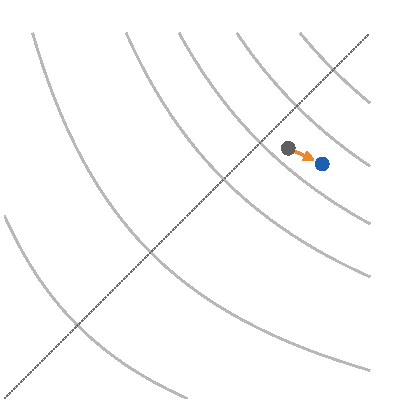
\includegraphics[width=0.8\linewidth]{figures/f1-poziomice.pdf}
\end{center}
{\footnotesize Płaszczyzna precyzja (poziom) -- czułość (pion), od $0{,}5$ do $1$, z poziomicami F1 (szare linie, od $0{,}6$ do $0{,}95$; kropkowana to $P=R$). Szara kropka: dekoder domyślny ($P=88{,}8\%$, $R=84{,}2\%$), niebieska: dostrojony ($93{,}5\%$, $82{,}1\%$); strzałka pokazuje zmianę.
Precyzja rośnie o $4{,}7$ punktu, czułość spada o $2{,}1$, a punkt przechodzi na wyższą poziomicę (F1 ze średnich $P,R$: $86{,}5\%\to87{,}4\%$); F1 jest tym większe, im bliżej górnego prawego rogu i im bliżej przekątnej. Raportowane makro-F1 ($85{,}9\%\to86{,}6\%$) jest liczone inaczej (przykład~\ref{prz:makro-mikro}).}\par\bigskip\hrule
\clearpage
\par\vspace{4mm}\noindent{\Large\bfseries Rysunek 17.2}\quad{\small(plik: rozdzial-17.tex)}\par\smallskip
\begin{center}

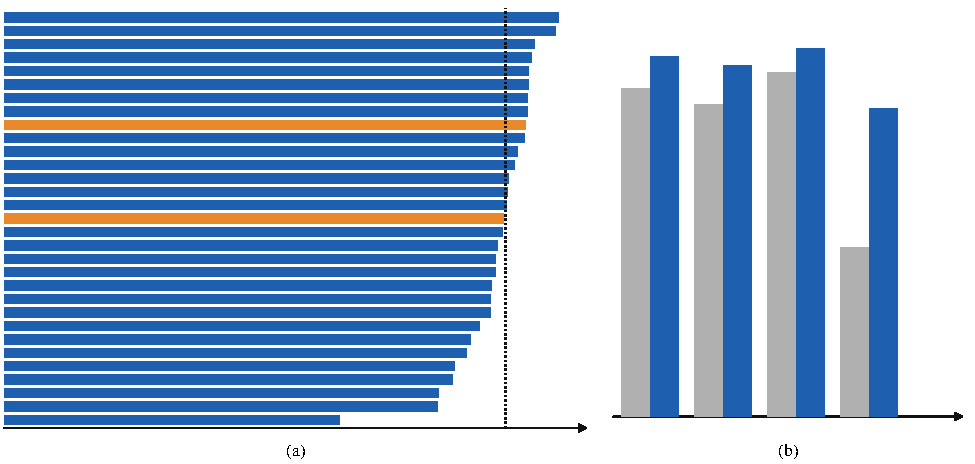
\includegraphics[width=0.8\linewidth]{figures/wyniki-grupy.pdf}
\end{center}
{\footnotesize (a) F1 nut (makro) dla każdej z $31$ grup testowych modelu końcowego (dekoder domyślny), od najlepszej do najgorszej; pomarańczowe słupki to prawdziwa gitara (GuitarSet), niebieskie --- syntetyczne nagrania klasyki; kropkowana pionowa to wynik ogólny $85{,}94\%$.
Najlepsze: pizzicato ($95{,}0\%$), ukulele ($94{,}5\%$), gitara klasyczna ($90{,}9\%$, $n=74$); najsłabsze: chór ($57{,}5\%$), wiolonczela ($74{,}3\%$), syntezator ($74{,}3\%$). (b) Gen~5 (szare) i Gen~6 (niebieskie) na GuitarSet: F1 nut razem, akompaniament, melodie, nuty z końcem (od lewej).}\par\bigskip\hrule

\par\vspace{4mm}\noindent{\Large\bfseries Rysunek 18.1}\quad{\small(plik: rozdzial-18.tex)}\par\smallskip
\begin{center}

\begin{tikzpicture}[>=Stealth,font=\footnotesize]
  \tikzset{b/.style={blok,text width=15mm,minimum width=15mm,inner sep=1.5pt,minimum height=12mm,align=center,font=\scriptsize},
           k/.style={font=\scriptsize,text=black!70,align=center}}
  \node[b] (w) at (0,0) {fala $x$\\$N$ próbek};
  \node[b,right=3.2mm of w] (h) {HCQT\\(rozdz.~7)};
  \node[b,right=3.2mm of h,fill=blue!8!white] (c) {trzon, $3\times$ blok\\(rozdz.~13)};
  \node[b,right=3.2mm of c,fill=blue!8!white] (z) {zejście $+\,e_s$\\(rozdz.~13)};
  \node[b,right=3.2mm of z,fill=orange!10!white] (x) {$2\times$ kontekst\\(rozdz.~14)};
  \node[b,right=3.2mm of x,fill=green!8!white] (g) {głowice\\(rozdz.~14)};
  \node[b,right=3.2mm of g] (d) {dekoder\\(rozdz.~16)};
  \node[b,right=3.2mm of d] (n) {lista nut\\$(m,t_0,t_1,i)$};
  \foreach \a/\bb in {w/h,h/c,c/z,z/x,x/g,g/d,d/n} {\draw[wektor] (\a)--(\bb);}
  \node[k,below=1mm of w] {$[N]$};
  \node[k,below=1mm of h] {$[9,T,159]$};
  \node[k,below=1mm of c] {$[48,T,159]$};
  \node[k,below=1mm of z] {$[T,53,64]$};
  \node[k,below=1mm of x] {$[T,53,64]$};
  \node[k,below=1mm of g] {$[T,53]{\times}4$\\$[T,6,21]$};
  \node[k,below=1mm of d] {progi\\$\theta_\mathrm{on},\dots$};
  \node[k,below=1mm of n] {MIDI,\\tabulatura};
\end{tikzpicture}
\end{center}
{\footnotesize Cała droga od fali do listy nut z kształtami tensorów (liczby zmierzone na prawdziwym modelu dla $T=243$ w tab.~\ref{tab:ksztalty}). Pola niebieskie to część konwolucyjna, pomarańczowe --- kontekst z uwagą, zielone --- głowice; dekoder nie ma parametrów uczonych gradientem.}\par\bigskip\hrule
\clearpage
\par\vspace{4mm}\noindent{\Large\bfseries Rysunek 18.2}\quad{\small(plik: rozdzial-18.tex)}\par\smallskip
\begin{center}

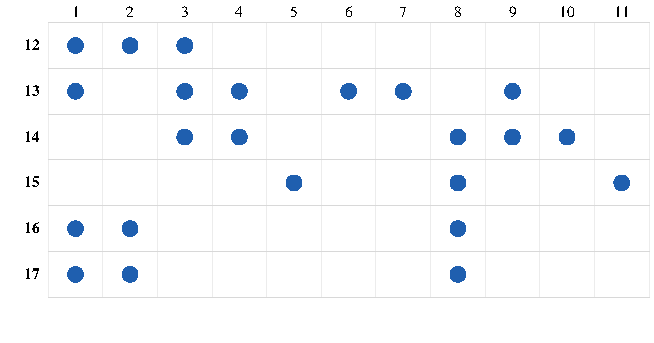
\includegraphics[width=0.8\linewidth]{figures/zaleznosci.pdf}
\end{center}
{\footnotesize Macierz zależności książki. Poziomo --- rozdziały matematyki i narzędzi ($1$--$11$), pionowo --- rozdziały o modelu ($12$--$17$); niebieska kropka oznacza, że rozdział o modelu wymaga danego rozdziału matematyki.
Np.\ blok harmoniczny (rozdz.~13) wymaga alikwotów ($3$), widma i HCQT ($6$, $7$), macierzy ($4$) i konwolucji ($9$); uczenie (rozdz.~15) --- pochodnych ($5$), straty ($8$) i optymalizacji ($11$).}\par\bigskip\hrule

\end{document}